% 'draft' mode can be used to speed up compilation
\documentclass[twoside,final]{hcmut-report}
\usepackage{codespace}

% Encodings
\usepackage{gensymb,textcomp}

% Better tables
\usepackage{array,longtable,multicol,multirow,siunitx,tabularx}

% Better enum
\usepackage{enumitem}

% Graphics
\usepackage{caption,float}

% Add options for figures, like max width, framing, etc.
\usepackage[export]{adjustbox}

% References
\usepackage[nameinlink]{cleveref}

% Configurations
\coursename{Deep Learning and Its Applications}
\reporttype{Assignment 2 -- Final Report}
\title{PASCAL VOC 2007 Object Detection}
\advisor{& Lê Thành Sách &}
\stuname{%
  & Trần Gia Lâm (Leader) & 2352670 \\
  & Nguyễn Hữu Cầu & 2352129 \\
}

% Prevent overfull lines on long monospace identifiers
\setlength{\emergencystretch}{3em}

% Set depth of numbering for counters
\AtBeginDocument{\counterwithin{lstlisting}{section}}

\begin{document}
\coverpage

\section*{Abstract}
\addcontentsline{toc}{section}{Abstract}
Object detection in unconstrained natural scenes requires joint spatial localization and multi-instance classification across severe scale variations and class imbalance. In this Assignment 2 Final Report for CO3133 (Semester 261, Group G-M10), we build a reproducible, leak-free PyTorch/Torchvision detection pipeline on the PASCAL VOC 2007 benchmark (20 foreground classes). Following task-specific Exploratory Data Analysis (EDA) on the official \texttt{VOCtrainval\_06-Nov-2007.tar} pool (5,011 images, 15,662 bounding boxes), we resolve a cross-split perceptual near-duplicate pair (\texttt{000863}/\texttt{008364}, $\text{dHash}=3$) to lock a leak-free stratified split of 4,014 training images (10,016 non-difficult boxes) and 997 validation images (2,592 non-difficult boxes, with 619 \texttt{difficult=1} boxes ignored per VOC2007 protocol).

We compare a lightweight single-stage baseline (\texttt{ssdlite320}, MobileNetV3-Large, 4.03M parameters, $320\times320$ input) against a pretrained two-stage Feature Pyramid detector (\texttt{Faster R-CNN ResNet-50-FPN}, \texttt{COCO\_V1}, 41.40M parameters, $640\text{--}1000\text{ px}$ input), and conduct a controlled study isolating backbone freezing (\texttt{fasterrcnn\_frozen}, 17.94M trainable parameters) versus full end-to-end fine-tuning (\texttt{fasterrcnn\_finetune}, 41.40M trainable parameters) under identical split, seed (42), initial predictor head weights, batch size (2), and SGD schedule ($\text{lr}=0.005$, no warmup). On our M3 NVIDIA L4 run, \texttt{fasterrcnn\_frozen} achieves \textbf{83.58\% validation mAP@0.5} (matching our M2 A100 run at 83.63\%), outperforming \texttt{ssdlite320} (50.70\% Val) by +32.88 percentage points and \texttt{fasterrcnn\_finetune} (75.51\% Val) by +8.07 percentage points while using 64.95\% less peak VRAM (1,266.2 MB vs. 3,612.2 MB). After auditing overlap against the official \texttt{VOCtest\_06-Nov-2007.tar} test set (4,952 images, 12,032 non-difficult objects; 0 ID overlap, 0 exact SHA-256 overlap), single-shot evaluation of the validation-selected checkpoints achieves \textbf{83.65\% Official Test mAP@0.5} for \texttt{fasterrcnn\_frozen}, \textbf{76.90\%} for \texttt{fasterrcnn\_finetune}, and \textbf{52.98\%} for \texttt{ssdlite320}. Size-stratified test evaluation confirms our EDA hypothesis: \texttt{ssdlite320} collapses on small objects ($<2\%$ image area) at 0.79\% AP@0.5, whereas \texttt{fasterrcnn\_frozen} achieves 45.32\% AP@0.5 and 92.61\% overall recall at $\text{score}\ge 0.30$.

\clearpage
\tableofcontents

\clearpage
\section{Problem Formulation, Dataset \& EDA}

\subsection{\textbf{Problem Statement and Task Definition}}
Given an arbitrary-resolution RGB photograph $I \in [0, 1]^{3 \times H \times W}$, the object detection model predicts a variable-length set of $N$ candidate detections:
\[
\hat{\mathcal{Y}} = \left\{ \left(\hat{\mathbf{b}}_i, \hat{c}_i, \hat{s}_i\right) \right\}_{i=1}^{N},
\]
where $\hat{\mathbf{b}}_i = (x_{\min,i}, y_{\min,i}, x_{\max,i}, y_{\max,i}) \in \mathbb{R}^4$ denotes the axis-aligned bounding box in absolute pixel coordinates ($0 \le x_{\min,i} < x_{\max,i} \le W$, $0 \le y_{\min,i} < y_{\max,i} \le H$), $\hat{c}_i \in \{1, 2, \dots, 20\}$ is the predicted foreground category across the 20 PASCAL VOC classes (\texttt{0} reserved for background), and $\hat{s}_i \in [0, 1]$ is the confidence score.

Our objectives in Assignment 2 are threefold:
\begin{enumerate}
    \item Build an end-to-end, leak-free PyTorch/Torchvision detection pipeline with automated bounding-box validity checks and a unit-tested VOC 2007 11-point interpolated $\text{mAP}@0.5$ evaluator.
    \item Compare a lightweight mobile single-stage detector (\texttt{ssdlite320}) against a pretrained two-stage Feature Pyramid detector (\texttt{Faster R-CNN ResNet-50-FPN}).
    \item Conduct a controlled experiment isolating \textbf{backbone freezing vs. full end-to-end fine-tuning} while holding the data split, random seed, initial 21-class predictor weights, batch size, optimizer, and learning-rate schedule strictly fixed, followed by a single-shot evaluation on the official VOC 2007 test set.
\end{enumerate}

\subsection{\textbf{Dataset Provenance, Finalized Split \& Overlap Audit}}
We use the official PASCAL Visual Object Classes Challenge 2007 (VOC2007) release:
\begin{itemize}
    \item \textbf{Trainval Pool:} \texttt{VOCtrainval\_06-Nov-2007.tar} (MD5 \texttt{c52e279531787c972589f7e41ab4ae64}), containing 5,011 images and 15,662 annotated bounding boxes (12,608 non-difficult and 3,054 marked \texttt{difficult=1}). No image-level subsampling was performed.
    \item \textbf{Official Test Set:} \texttt{VOCtest\_06-Nov-2007.tar} (MD5 \texttt{b6e924de25625d8de591ea690078ad9f}), containing 4,952 test images and 14,976 annotated boxes (12,032 non-difficult and 2,944 \texttt{difficult=1} ignored).
    \item \textbf{Near-Duplicate Leak Resolution:} During M1 EDA, perceptual hashing identified a cross-split near-duplicate pair: \texttt{000863} (originally in \texttt{val}) and \texttt{008364} (in \texttt{train}), with $\text{dHash}=3$ and $\text{aHash}=2$. Prior to training, we grouped \texttt{000863} into \texttt{train}, yielding a leak-free split with fingerprint \texttt{split\_sha256 = c60294fe...139c2bd6c}.
    \item \textbf{Trainval-vs-Test Overlap Audit (\texttt{test\_overlap\_check.json}):} Comparing all 5,011 \texttt{trainval} images against all 4,952 \texttt{test} images yields \textbf{0 image ID overlaps}, \textbf{0 exact SHA-256 byte overlaps}, and 59 low-variance perceptual hash collisions ($\text{dHash}\le 4$, primarily uniform sky/horizon backgrounds such as \texttt{003183}).
\end{itemize}

\begin{table}[H]
\centering
\caption{Finalized PASCAL VOC 2007 Dataset Partitions and Difficult-Object Policy}
\resizebox{\linewidth}{!}{%
\begin{tabular}{lrrrrr}
\toprule
\textbf{Partition} & \textbf{Images} & \textbf{All Boxes} & \textbf{Non-Difficult (\texttt{diff=0})} & \textbf{Difficult (\texttt{diff=1})} & \textbf{Leakage Status} \\
\midrule
Official \texttt{trainval} pool & 5,011 & 15,662 & 12,608 & 3,054 & --- \\
Training (\texttt{splits/train.txt}) & 4,014 & 12,451 & 10,016 & 2,435 & 0 cross-split dups \\
Validation (\texttt{splits/val.txt}) & 997 & 3,211 & 2,592 & 619 (ignored) & 0 cross-split dups \\
Official Test (\texttt{test.txt}) & 4,952 & 14,976 & 12,032 & 2,944 (ignored) & 0 ID / 0 SHA-256 overlap \\
\bottomrule
\end{tabular}%
}
\end{table}

\subsection{\textbf{Task-Specific Exploratory Data Analysis (EDA)}}
\begin{figure}[H]
    \centering
    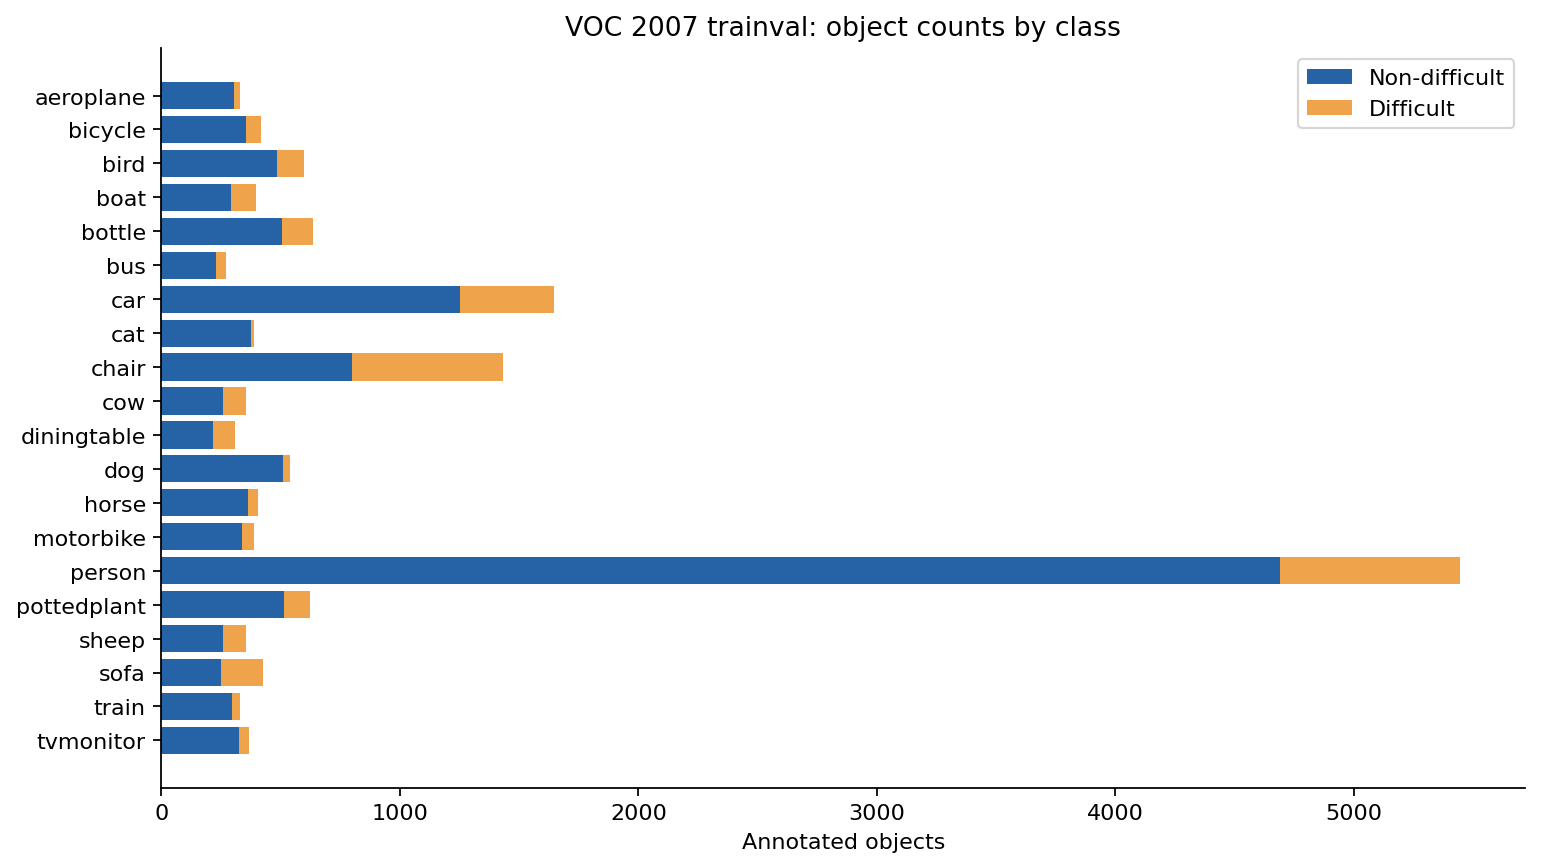
\includegraphics[width=0.88\linewidth]{../../../a2_m1/outputs/a2_eda/20261006T225426_686818Z/figures/class_distribution.png}
    \caption{Per-class instance distribution across the 20 PASCAL VOC 2007 foreground classes.}
\end{figure}

\begin{figure}[H]
    \centering
    \begin{minipage}{0.48\linewidth}
        \centering
        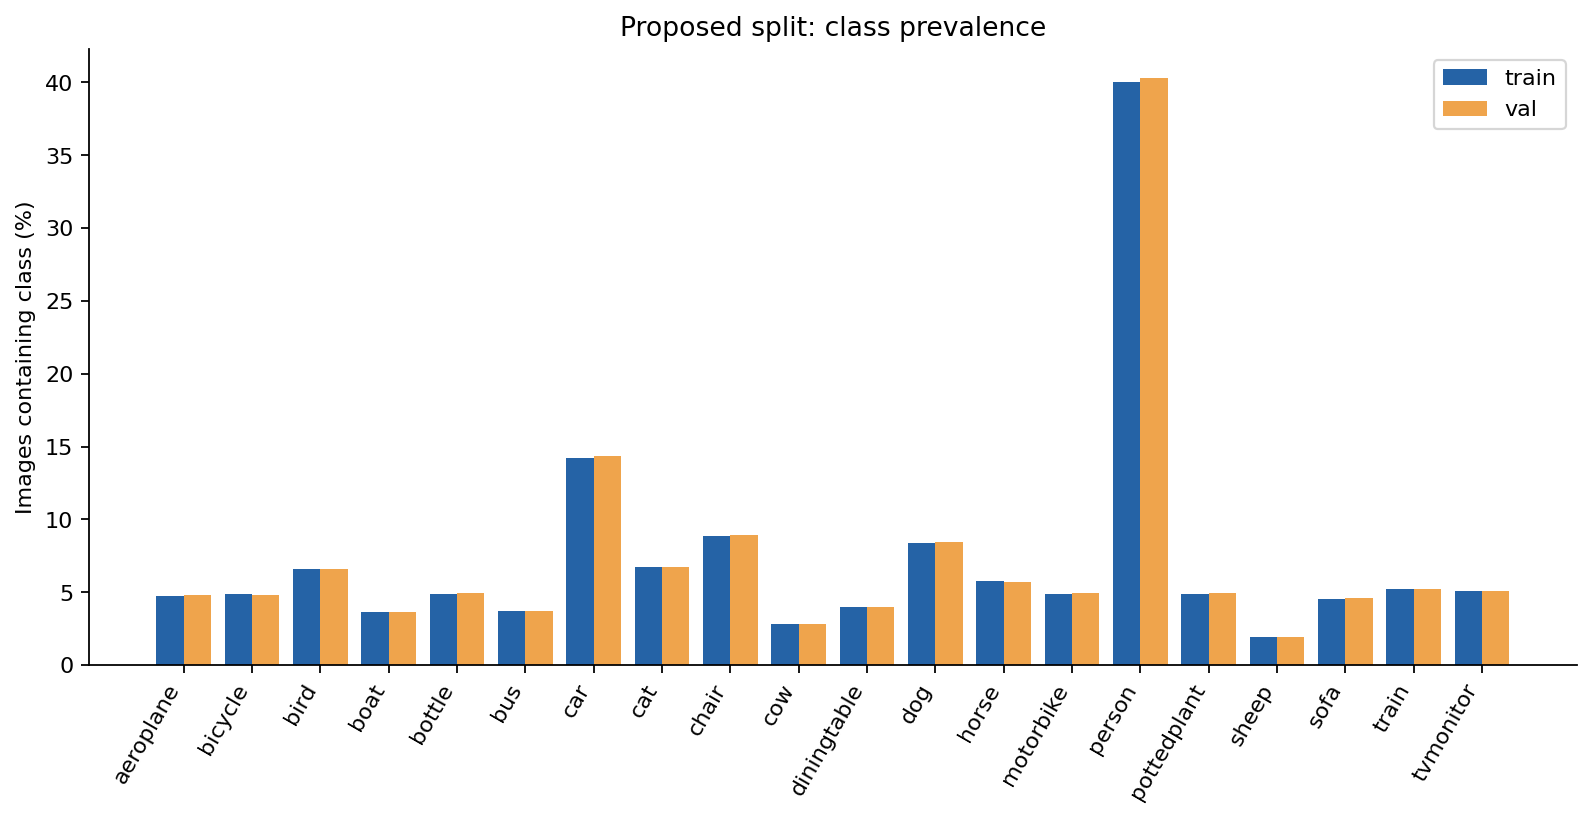
\includegraphics[width=\linewidth]{../../../a2_m1/outputs/a2_eda/20261006T225426_686818Z/figures/split_class_prevalence.png}
        \caption{Train vs. validation class prevalence.}
    \end{minipage}\hfill
    \begin{minipage}{0.48\linewidth}
        \centering
        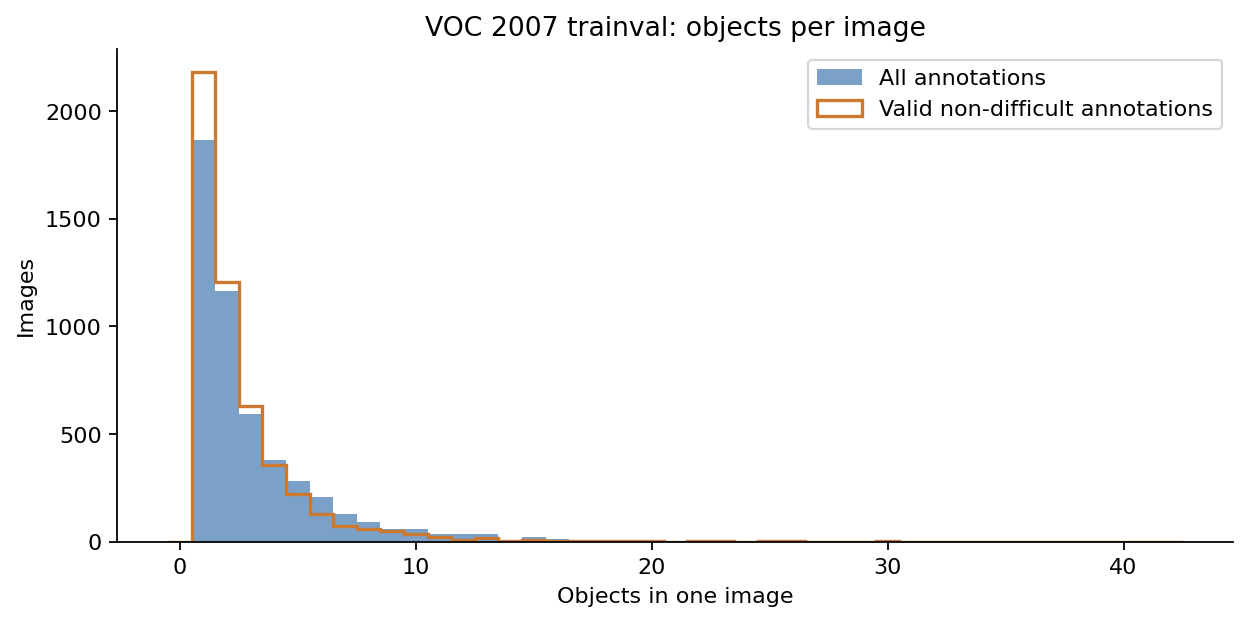
\includegraphics[width=\linewidth]{../../../a2_m1/outputs/a2_eda/20261006T225426_686818Z/figures/objects_per_image.png}
        \caption{Objects per image distribution.}
    \end{minipage}
\end{figure}

\begin{figure}[H]
    \centering
    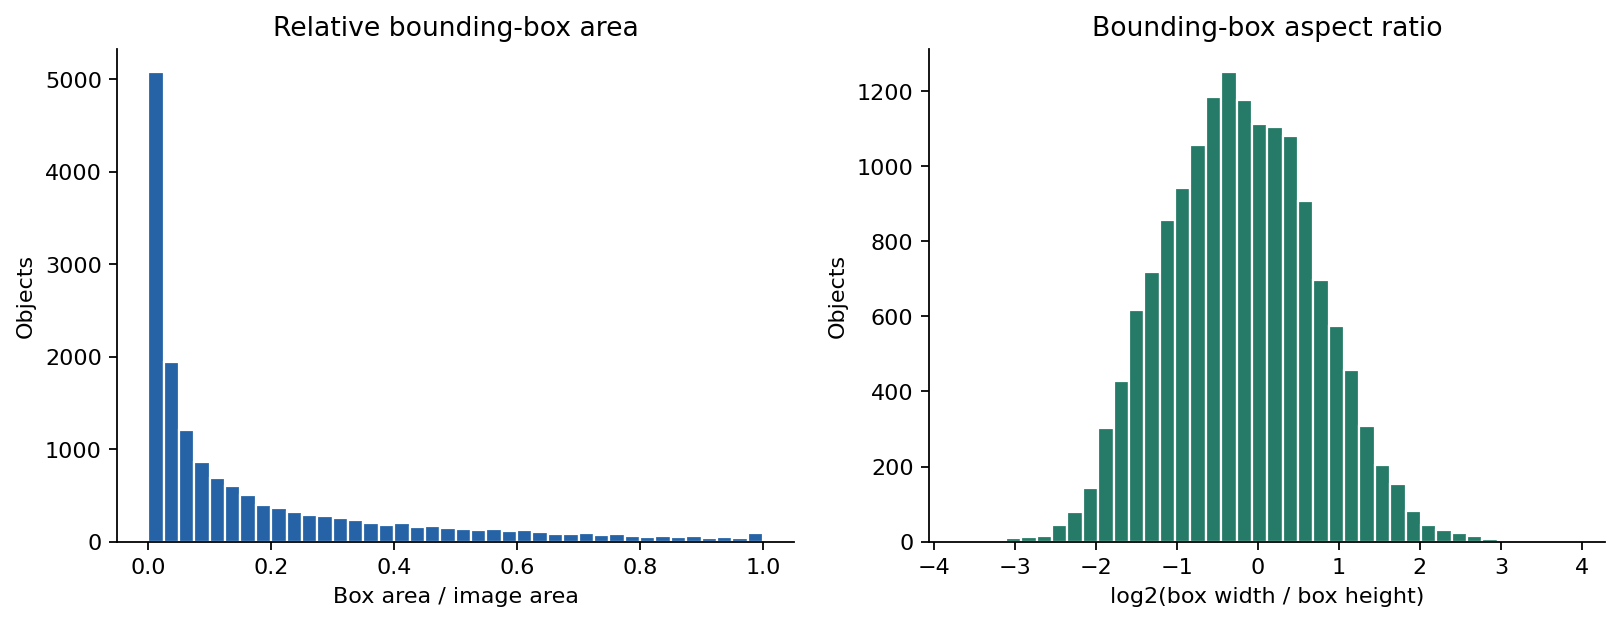
\includegraphics[width=0.88\linewidth]{../../../a2_m1/outputs/a2_eda/20261006T225426_686818Z/figures/bbox_size_distribution.png}
    \caption{Relative bounding-box area and aspect ratio distribution across 12,608 non-difficult boxes.}
\end{figure}

Our EDA reveals four structural properties of VOC 2007 that directly motivate our modeling decisions:
\begin{enumerate}
    \item \textbf{Severe Class Imbalance ($22.02 : 1$):} \texttt{person} has 4,690 non-difficult instances, whereas \texttt{bus} (213), \texttt{diningtable} (215), \texttt{sofa} (248), and \texttt{sheep} (257) are scarce. Because $\text{mAP}@0.5$ averages AP equally across all 20 classes, strong representations for rare classes are essential.
    \item \textbf{Small-Object Bottleneck (EDA Hypothesis):} Across 12,608 non-difficult boxes, \textbf{2,597 boxes (20.60\%)} occupy $<2\%$ of the image area (small), 4,782 (37.93\%) occupy $2\text{--}15\%$ (medium), and 5,229 (41.47\%) occupy $\ge 15\%$ (large). Warping images to $320\times320$ in \texttt{ssdlite320} shrinks small objects below $45\times45$ px, whereas \texttt{Faster R-CNN ResNet-50-FPN} ($640\text{--}1000\text{ px}$ + multi-scale FPN \texttt{P2--P6}) preserves fine spatial resolution. We hypothesize \texttt{Faster R-CNN} will achieve its largest gains on small and medium objects.
    \item \textbf{Multi-Object Crowding:} Images average 2.52 non-difficult objects (max 37), with 36 training and 8 validation images containing only \texttt{difficult=1} annotations.
    \item \textbf{DataLoader \& Coordinate Verification:} \texttt{a2/data.py} converts RGB images to \texttt{float32} tensors in $[0,1]$, applies random horizontal flipping ($p=0.5$) during training with exact box reflection $x'_{\min}=W-x_{\max}$, $x'_{\max}=W-x_{\min}$, and asserts $x_{\max}>x_{\min}$, $y_{\max}>y_{\min}$ on every sample.
\end{enumerate}

\begin{figure}[H]
    \centering
    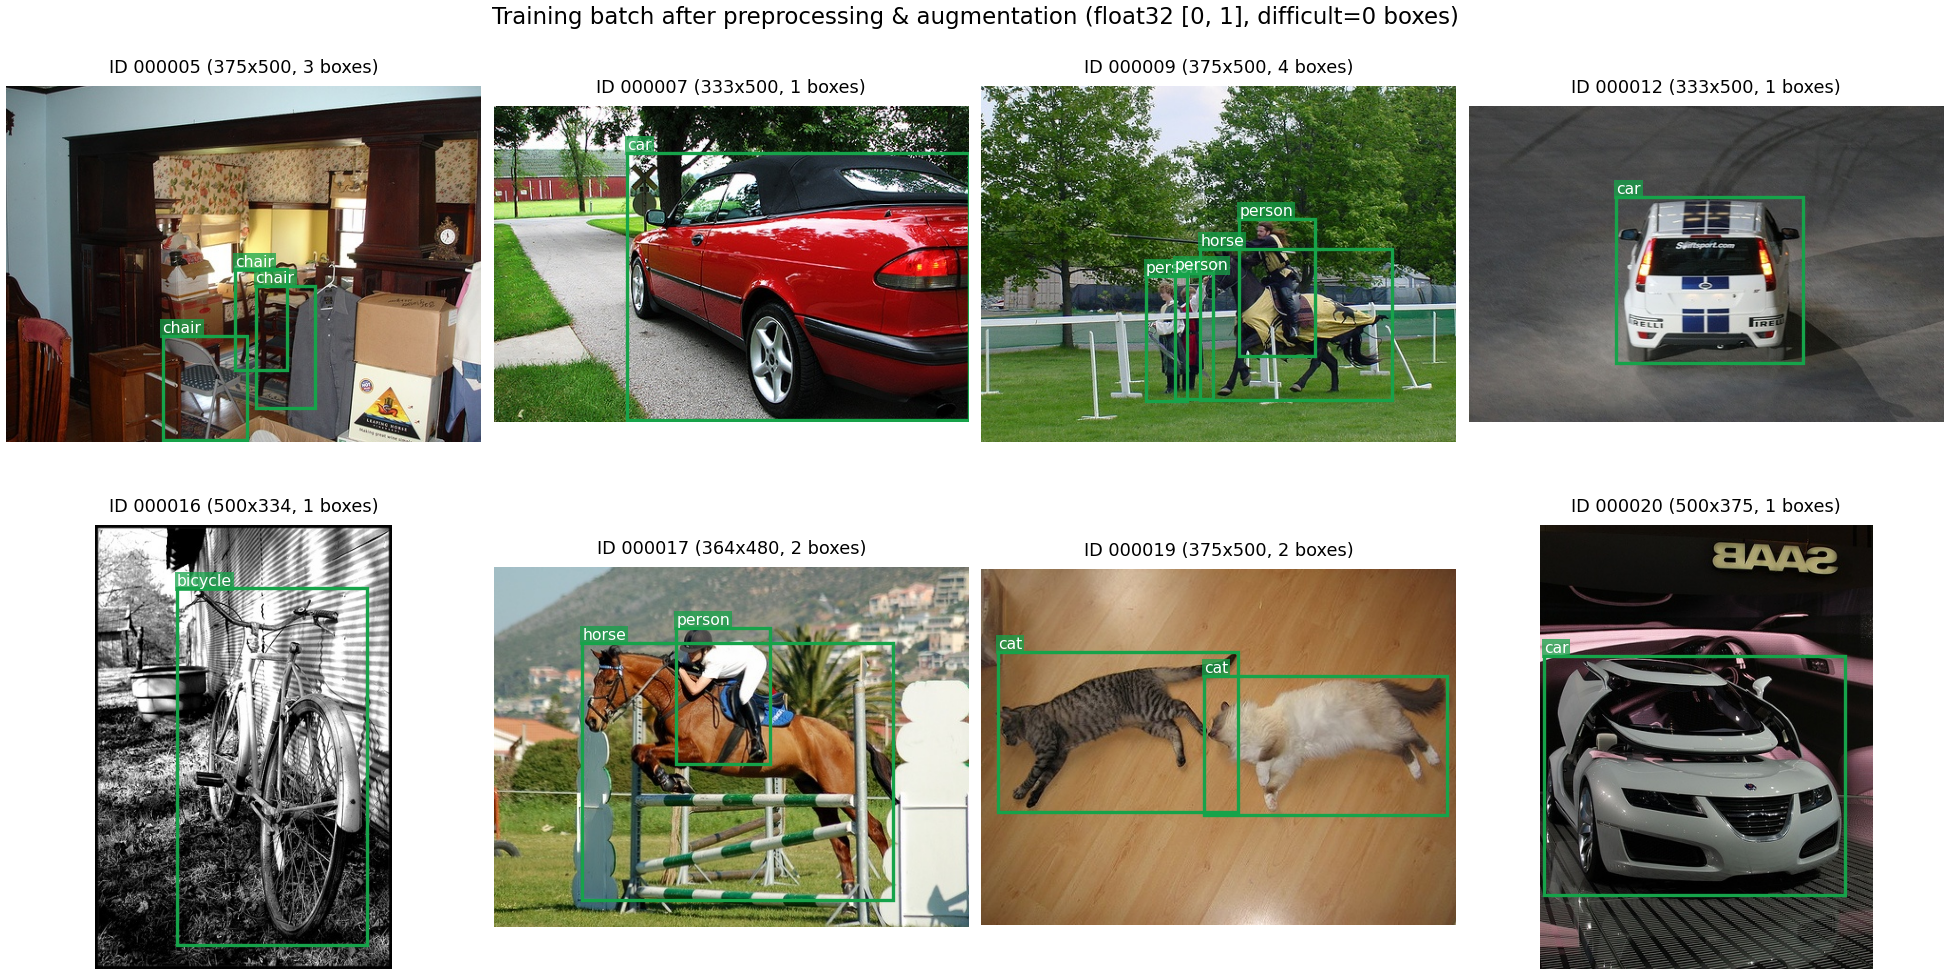
\includegraphics[width=0.88\linewidth]{../../outputs/a2_m3_a100/eda/batch_preview.png}
    \caption{Inspected training batch ($B=8$, image IDs \texttt{000005}--\texttt{000020}) after preprocessing and tensor conversion.}
\end{figure}

\section{Methodology \& Controlled Experiment}

\subsection{\textbf{End-to-End Pipeline and Model Configurations}}
\begin{figure}[H]
    \centering
    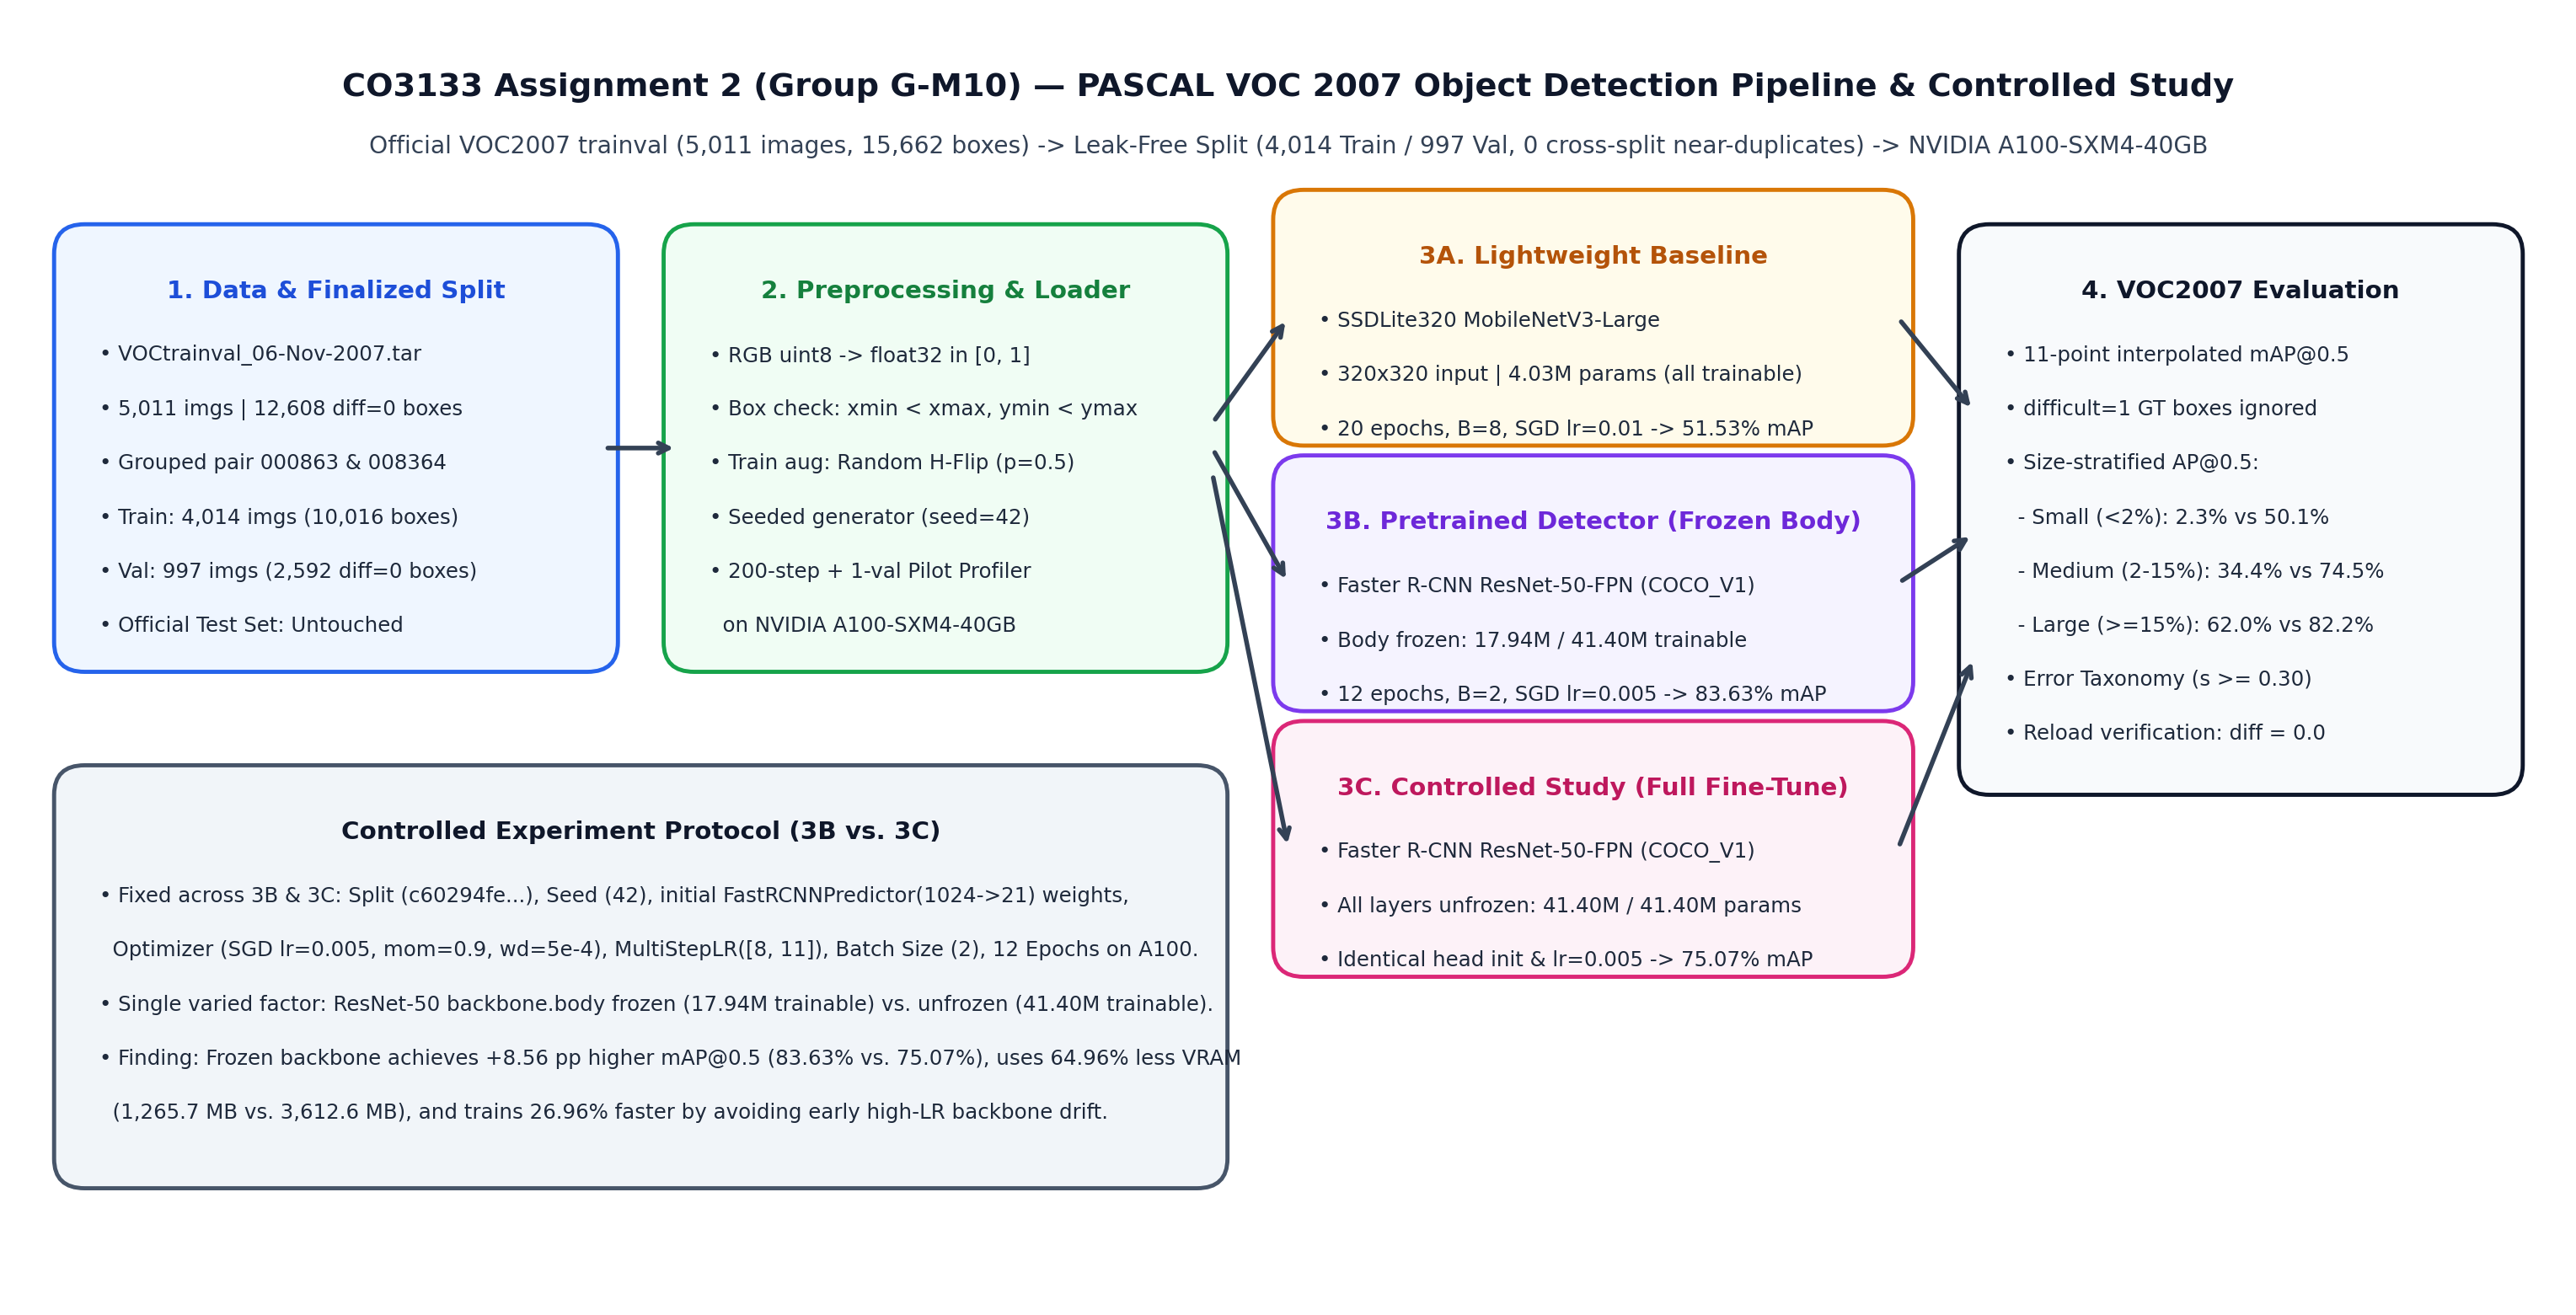
\includegraphics[width=0.92\linewidth]{../../assets/assignment2/pipeline.png}
    \caption{End-to-end PASCAL VOC 2007 object detection pipeline and controlled experiment design.}
\end{figure}

\begin{table}[H]
\centering
\caption{Model Architectures and Hyperparameter Protocol}
\resizebox{\linewidth}{!}{%
\begin{tabular}{llll}
\toprule
\textbf{Setting / Factor} & \textbf{\texttt{ssdlite320}} & \textbf{\texttt{fasterrcnn\_frozen}} & \textbf{\texttt{fasterrcnn\_finetune}} \\
\midrule
Family & Single-stage anchor & Two-stage FPN + RPN + RoI & Two-stage FPN + RPN + RoI \\
Backbone & MobileNetV3-Large & ResNet-50-FPN (\texttt{COCO\_V1}) & ResNet-50-FPN (\texttt{COCO\_V1}) \\
Varied Factor & All layers trainable & \texttt{backbone.body} FROZEN & \texttt{backbone.body} UNFROZEN \\
Trainable / Total Params & 4.03M / 4.03M (100\%) & 17.94M / 41.40M (43.3\%) & 41.40M / 41.40M (100\%) \\
Input Resolution & Fixed $320 \times 320$ & \texttt{min=640, max=1000} & \texttt{min=640, max=1000} \\
Optimizer & SGD ($\text{lr}=0.01$, wd $5\text{e-}4$) & SGD ($\text{lr}=0.005$, wd $5\text{e-}4$) & SGD ($\text{lr}=0.005$, wd $5\text{e-}4$) \\
LR Schedule & \texttt{MultiStepLR([12,16])} & \texttt{MultiStepLR([8,11])} & \texttt{MultiStepLR([8,11])} \\
Batch Size / Epochs & $B=8$ / 20 epochs & $B=2$ / 12 epochs & $B=2$ / 12 epochs \\
\bottomrule
\end{tabular}%
}
\end{table}

\subsection{\textbf{Controlled Experiment Protocol and Evaluation Metrics}}
Between \texttt{fasterrcnn\_frozen} and \texttt{fasterrcnn\_finetune}, we hold the data split, data order, random seed (42), initial \texttt{COCO\_V1} weights, newly initialized 21-class \texttt{FastRCNNPredictor} weights (seeded identically at 42 immediately before head replacement), batch size (2), gradient clipping ($\text{max\_norm}=10.0$), and SGD schedule ($\text{lr}=0.005$, no warmup) strictly fixed. The single varied factor is whether \texttt{backbone.body} (23,454,912 parameters) is frozen or updated.

We evaluate all models using the official PASCAL VOC 2007 11-point interpolated $\text{mAP}@0.5$ ($\text{IoU}\ge0.50$), ignoring detections matching \texttt{difficult=1} boxes, verified prior to execution via \texttt{self\_test\_voc\_evaluator()}. Checkpoints (\texttt{best.pt}) are selected strictly by highest validation $\text{mAP}@0.5$ before any official test-set evaluation.

\section{Experimental Results: Validation \& Official Test}

\subsection{\textbf{Compute Pilot (A100) and Validation Results (L4)}}
In M2, 200-batch + 1-validation-pass pilots on \texttt{NVIDIA A100-SXM4-40GB} profiled step time, VRAM, and early convergence: \texttt{ssdlite320} ($110.92\text{ ms/step}$, $462.6\text{ MB}$ VRAM, $8.81\%$ pilot mAP), \texttt{fasterrcnn\_frozen} ($77.55\text{ ms/step}$, $1,238.1\text{ MB}$ VRAM, \textbf{65.02\%} pilot mAP), and \texttt{fasterrcnn\_finetune} ($84.98\text{ ms/step}$, $3,325.9\text{ MB}$ VRAM, $35.81\%$ pilot mAP). In M3, the full pipeline (\texttt{all\_m3}) was executed on Google Colab \texttt{NVIDIA L4} (22.03 GB VRAM, PyTorch \texttt{2.14.1+cu130}), reproducing our M2 validation results within 0.05--0.83 pp.

\begin{table}[H]
\centering
\caption{M3 Validation Results at Selected Checkpoints (997 Validation Images, 2,592 Non-Difficult Boxes, NVIDIA L4)}
\resizebox{\linewidth}{!}{%
\begin{tabular}{lrrrrrrrrr}
\toprule
\textbf{Model} & \textbf{Best Ep} & \textbf{Val mAP} & \textbf{Small AP} & \textbf{Med AP} & \textbf{Large AP} & \textbf{Train (s)} & \textbf{Latency} & \textbf{VRAM} \\
\midrule
\texttt{ssdlite320} & 17 / 20 & 50.70\% & 1.85\% & 34.60\% & 63.29\% & 829.4 & 16.22 ms & 462.8 MB \\
\texttt{fasterrcnn\_frozen} & 11 / 12 & \textbf{83.58\%} & \textbf{50.10\%} & \textbf{74.36\%} & \textbf{81.71\%} & 2,425.1 & 31.34 ms & 1,266.2 MB \\
\texttt{fasterrcnn\_finetune} & 12 / 12 & 75.51\% & 42.50\% & 62.19\% & 75.22\% & 3,926.0 & 30.79 ms & 3,612.2 MB \\
\bottomrule
\end{tabular}%
}
\end{table}

\begin{figure}[H]
    \centering
    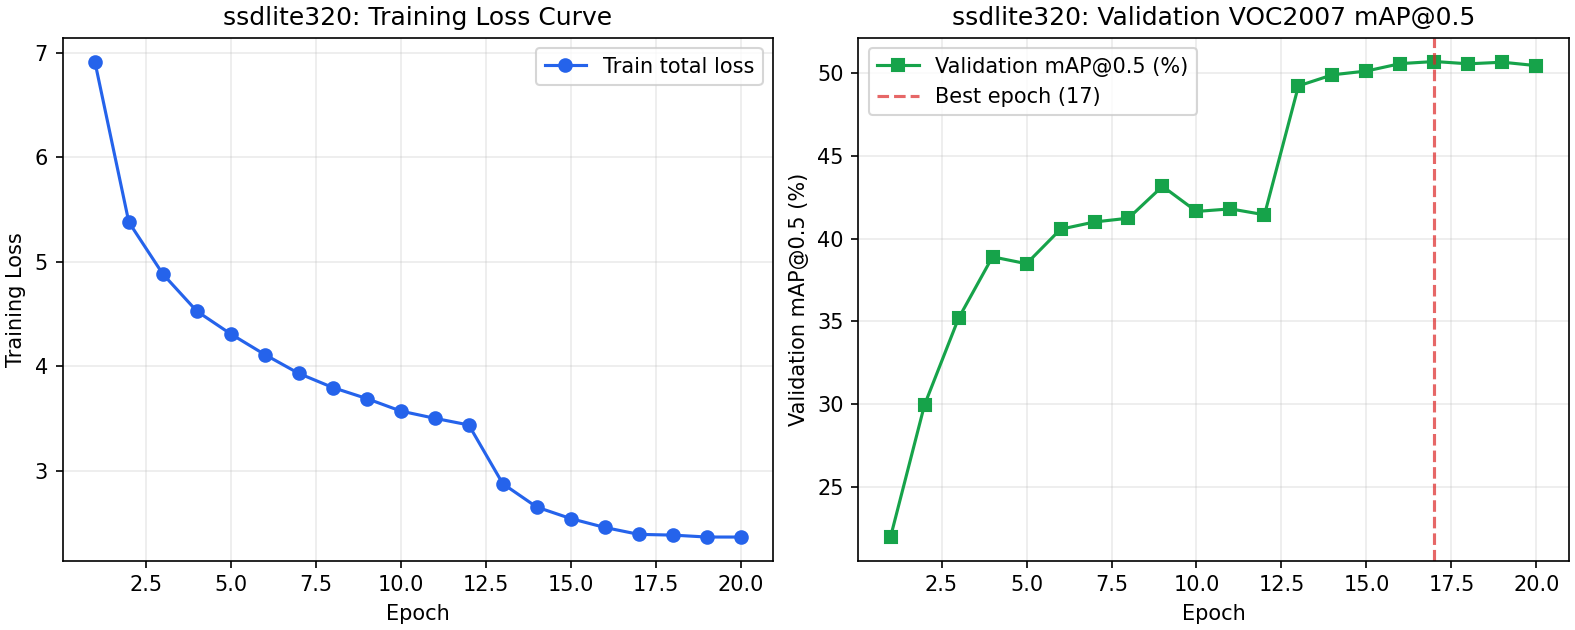
\includegraphics[width=0.82\linewidth]{../../outputs/a2_m3_a100/ssdlite320/curves.png}
    \caption{\texttt{ssdlite320} training loss and validation mAP@0.5 over 20 epochs (best: 50.70\% at epoch 17).}
\end{figure}

\begin{figure}[H]
    \centering
    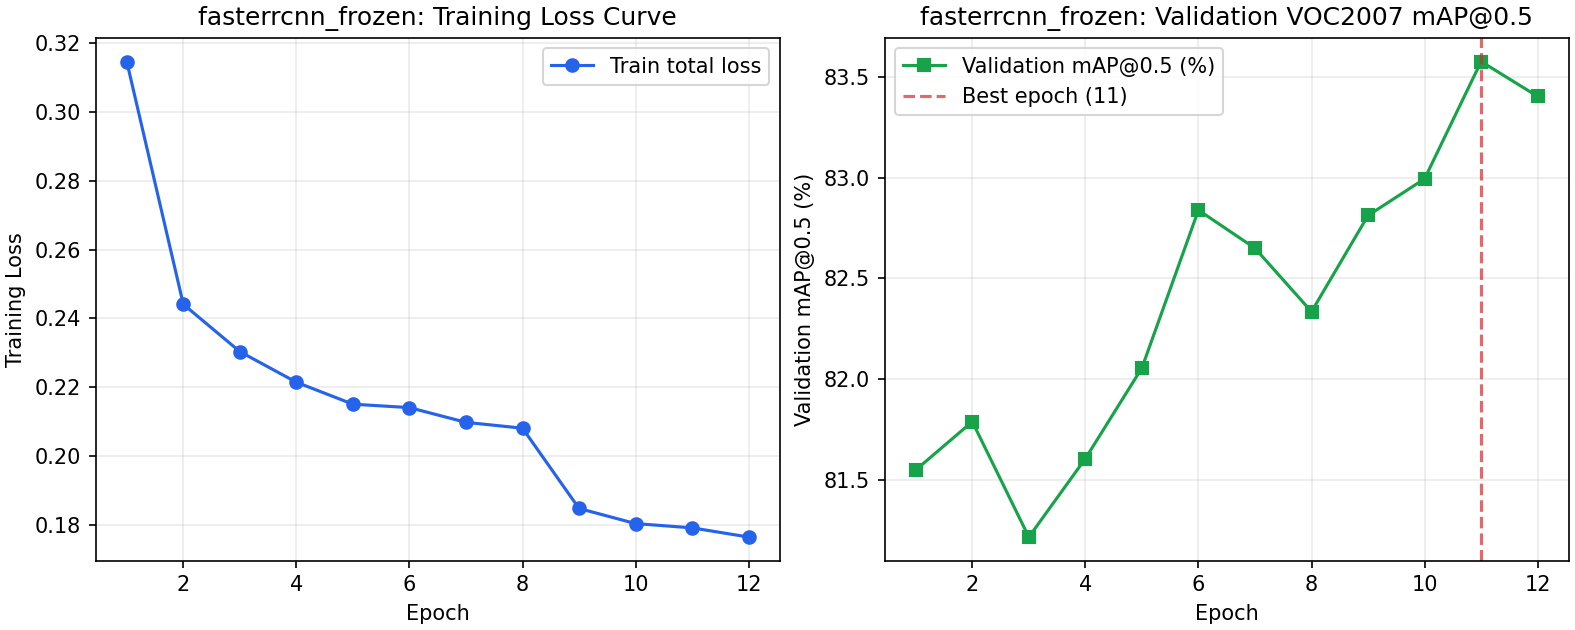
\includegraphics[width=0.82\linewidth]{../../outputs/a2_m3_a100/fasterrcnn_frozen/curves.png}
    \caption{\texttt{fasterrcnn\_frozen} curves over 12 epochs (best: 83.58\% at epoch 11).}
\end{figure}

\begin{figure}[H]
    \centering
    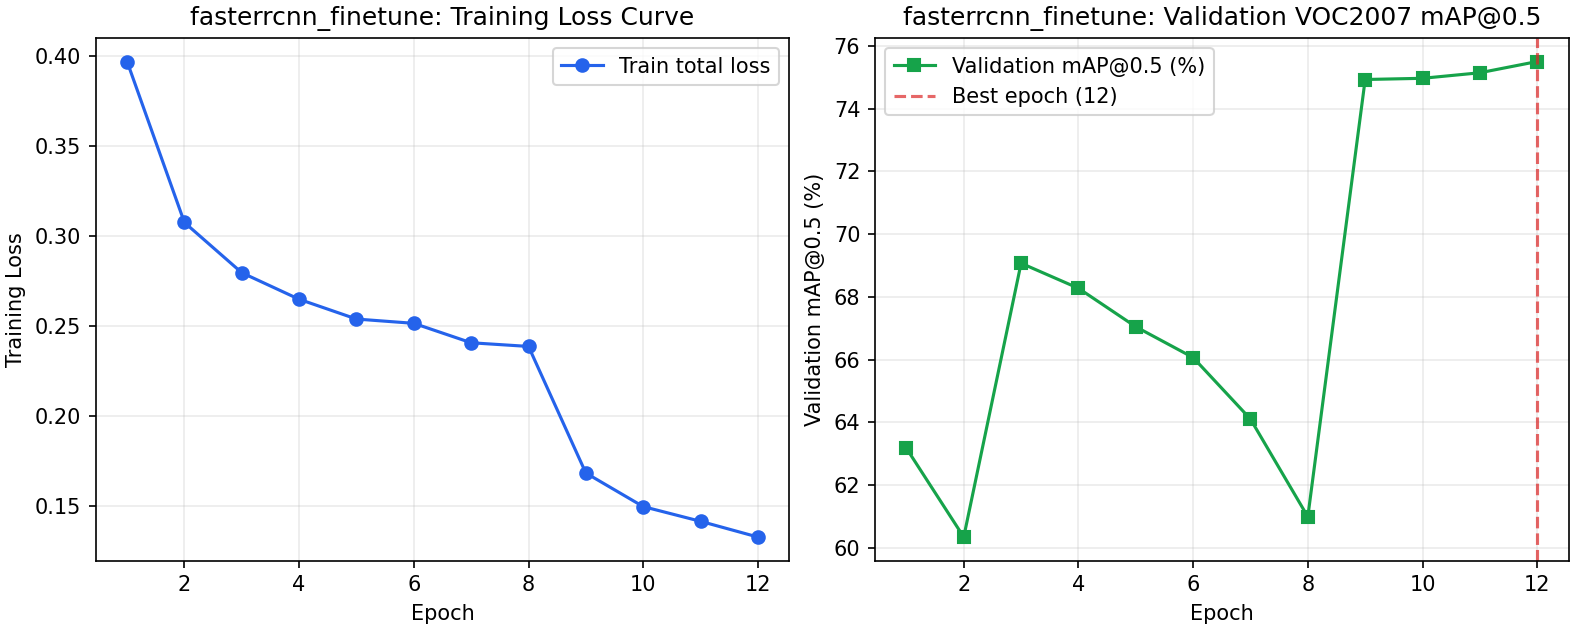
\includegraphics[width=0.82\linewidth]{../../outputs/a2_m3_a100/fasterrcnn_finetune/curves.png}
    \caption{\texttt{fasterrcnn\_finetune} curves over 12 epochs (best: 75.51\% at epoch 12; note instability in epochs 1--8).}
\end{figure}

\subsection{\textbf{Official VOC 2007 Test Set Evaluation (Single-Shot)}}
After locking all checkpoint selections on validation, each model's \texttt{best.pt} was evaluated once on the 4,952 official test images (12,032 non-difficult objects; 2,944 \texttt{difficult=1} ignored) of \texttt{VOCtest\_06-Nov-2007.tar}.

\begin{table}[H]
\centering
\caption{Validation vs. Official VOC 2007 Test Set Comparison (4,952 Test Images, 12,032 Non-Difficult Objects)}
\resizebox{\linewidth}{!}{%
\begin{tabular}{lrrrrrrr}
\toprule
\textbf{Model} & \textbf{Ep} & \textbf{Val mAP@0.5} & \textbf{Test mAP@0.5} & \textbf{Delta} & \textbf{Test Small} & \textbf{Test Med} & \textbf{Test Large} \\
\midrule
\texttt{ssdlite320} & 17 & 50.70\% & \textbf{52.98\%} & +2.28 pp & 0.79\% & 32.75\% & 64.98\% \\
\texttt{fasterrcnn\_frozen} & 11 & \textbf{83.58\%} & \textbf{83.65\%} & +0.07 pp & \textbf{45.32\%} & \textbf{75.15\%} & \textbf{81.89\%} \\
\texttt{fasterrcnn\_finetune} & 12 & 75.51\% & \textbf{76.90\%} & +1.40 pp & 32.89\% & 63.46\% & 76.36\% \\
\bottomrule
\end{tabular}%
}
\end{table}

Every model generalizes consistently from the 997-image validation split to the 4,952-image official test set: \texttt{fasterrcnn\_frozen} maintains virtually identical accuracy (83.58\% Val $\to$ \textbf{83.65\% Test}, +0.07 pp), outperforming \texttt{ssdlite320} by +30.67 pp and \texttt{fasterrcnn\_finetune} by +6.75 pp on the official benchmark.

\section{Error Analysis \& Compute Trade-Offs}

\subsection{\textbf{Official Test Error Taxonomy \texorpdfstring{($\text{score} \ge 0.30$)}{(score >= 0.30)}}}
\begin{table}[H]
\centering
\caption{Official Test Set Error Taxonomy across 12,032 Non-Difficult Ground-Truth Boxes ($\hat{s} \ge 0.30$)}
\resizebox{\linewidth}{!}{%
\begin{tabular}{lrrr}
\toprule
\textbf{Outcome / Error Category} & \textbf{\texttt{ssdlite320}} & \textbf{\texttt{fasterrcnn\_frozen}} & \textbf{\texttt{fasterrcnn\_finetune}} \\
\midrule
Correct Detections (TP) & 6,661 (55.36\%) & \textbf{11,143 (92.61\%)} & 10,108 (84.01\%) \\
Missed GT Objects (FN Total) & 5,371 (44.64\%) & \textbf{889 (7.39\%)} & 1,924 (15.99\%) \\
\quad $\hookrightarrow$ Missed Small GT ($<2\%$ area) & 2,151 & \textbf{367} & 750 \\
Wrong Class Error ($\text{IoU} \ge 0.50$) & 1,133 & \textbf{938} & 1,242 \\
Localization Error ($0.10 \le \text{IoU} < 0.50$) & 1,981 & 3,952 & 2,517 \\
Duplicate Detection & 494 & 814 & 538 \\
Background False Positive ($\text{IoU} < 0.10$) & 1,031 & 2,840 & 1,713 \\
\bottomrule
\end{tabular}%
}
\end{table}

\begin{figure}[H]
    \centering
    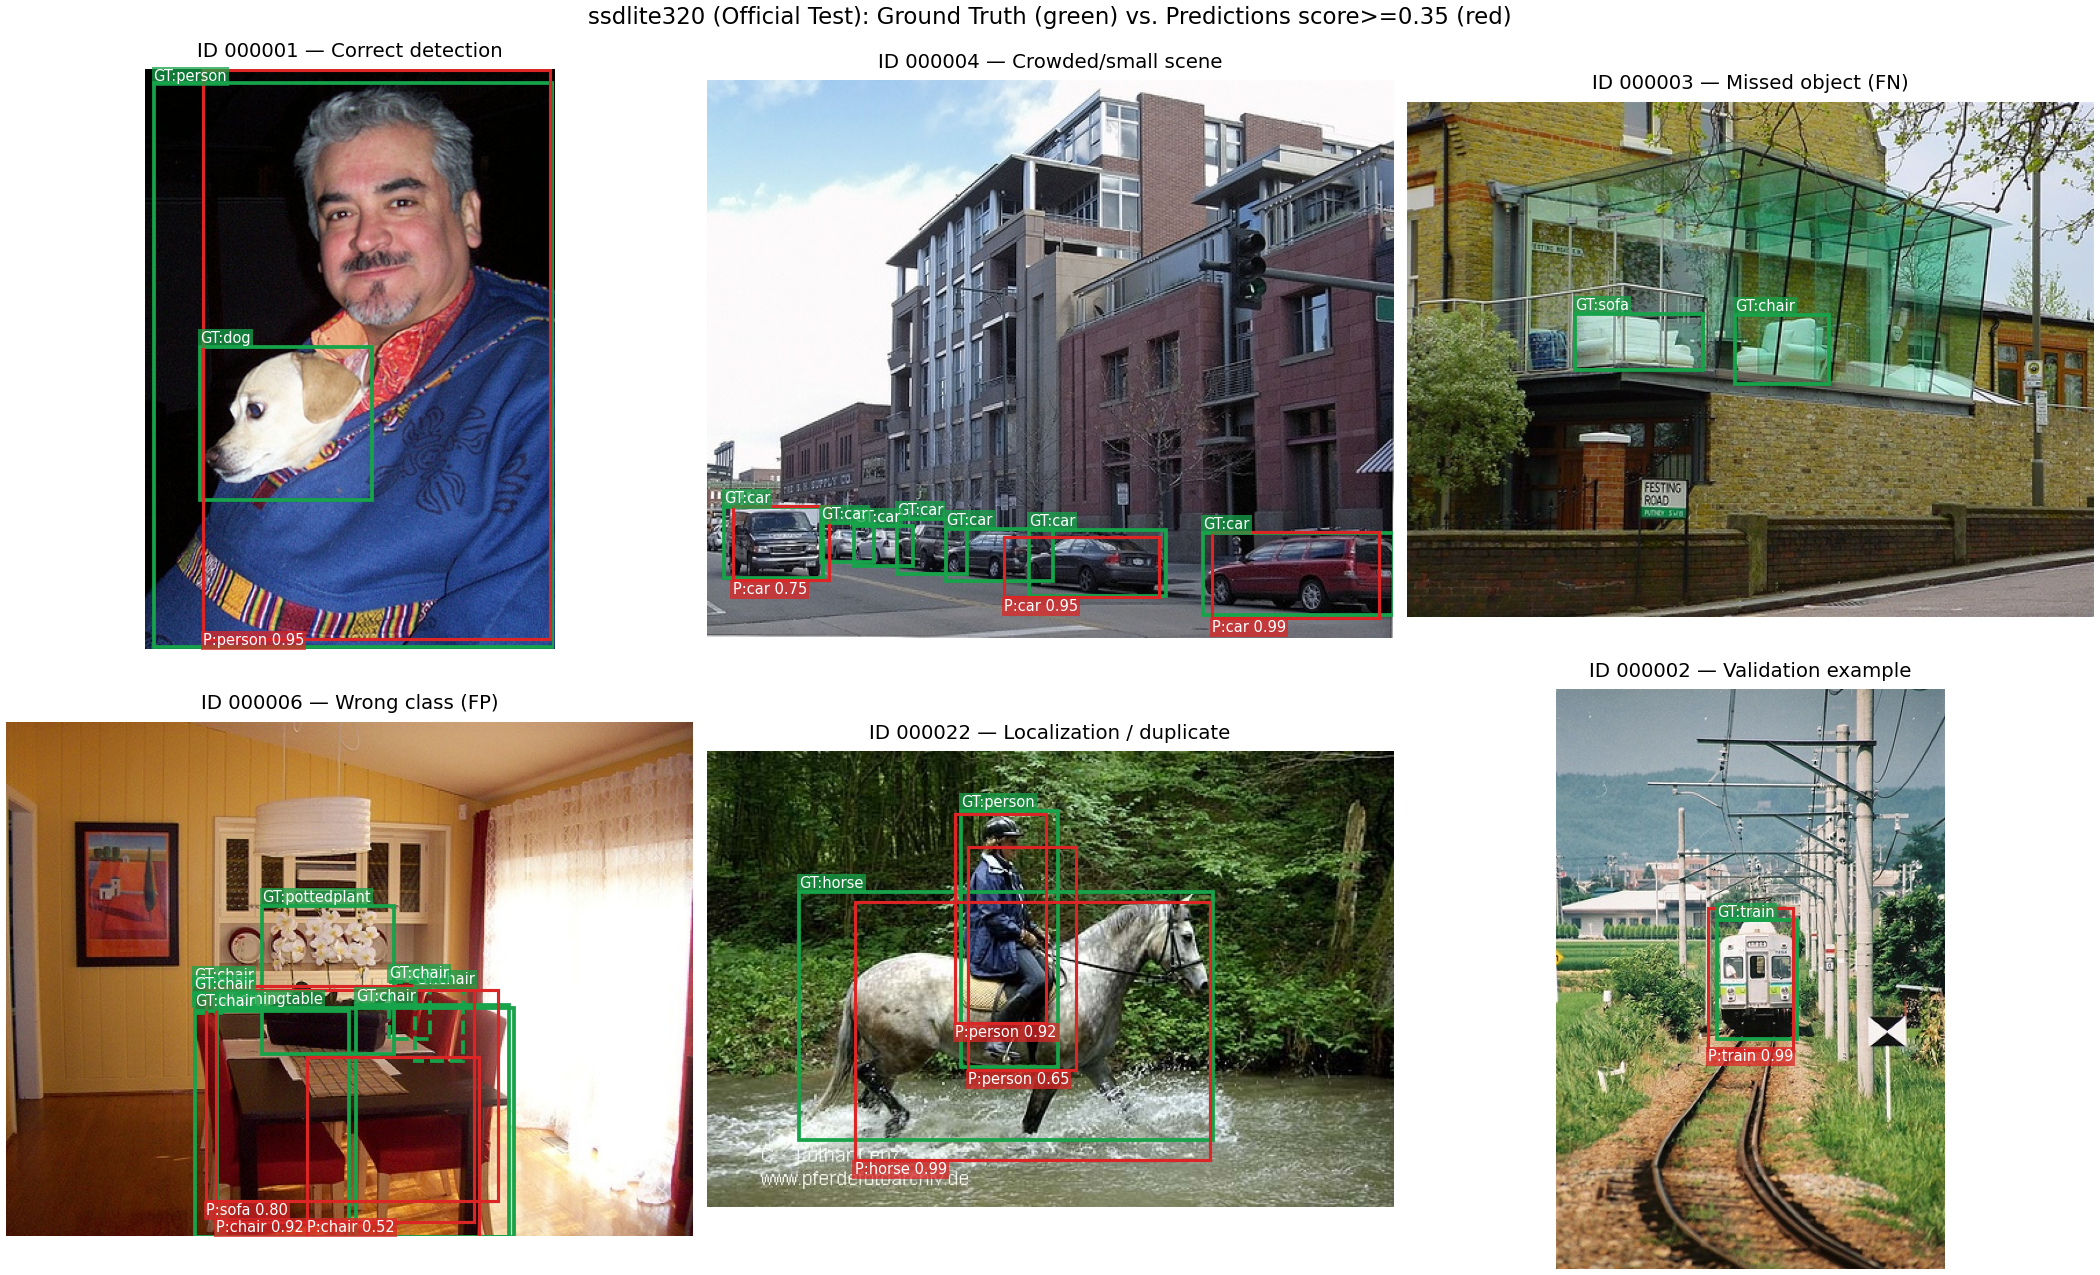
\includegraphics[width=0.90\linewidth]{../../outputs/a2_m3_a100/ssdlite320/test_examples.png}
    \caption{\texttt{ssdlite320} qualitative Official Test examples (green: GT, red: predictions $\ge 0.35$).}
\end{figure}

\begin{figure}[H]
    \centering
    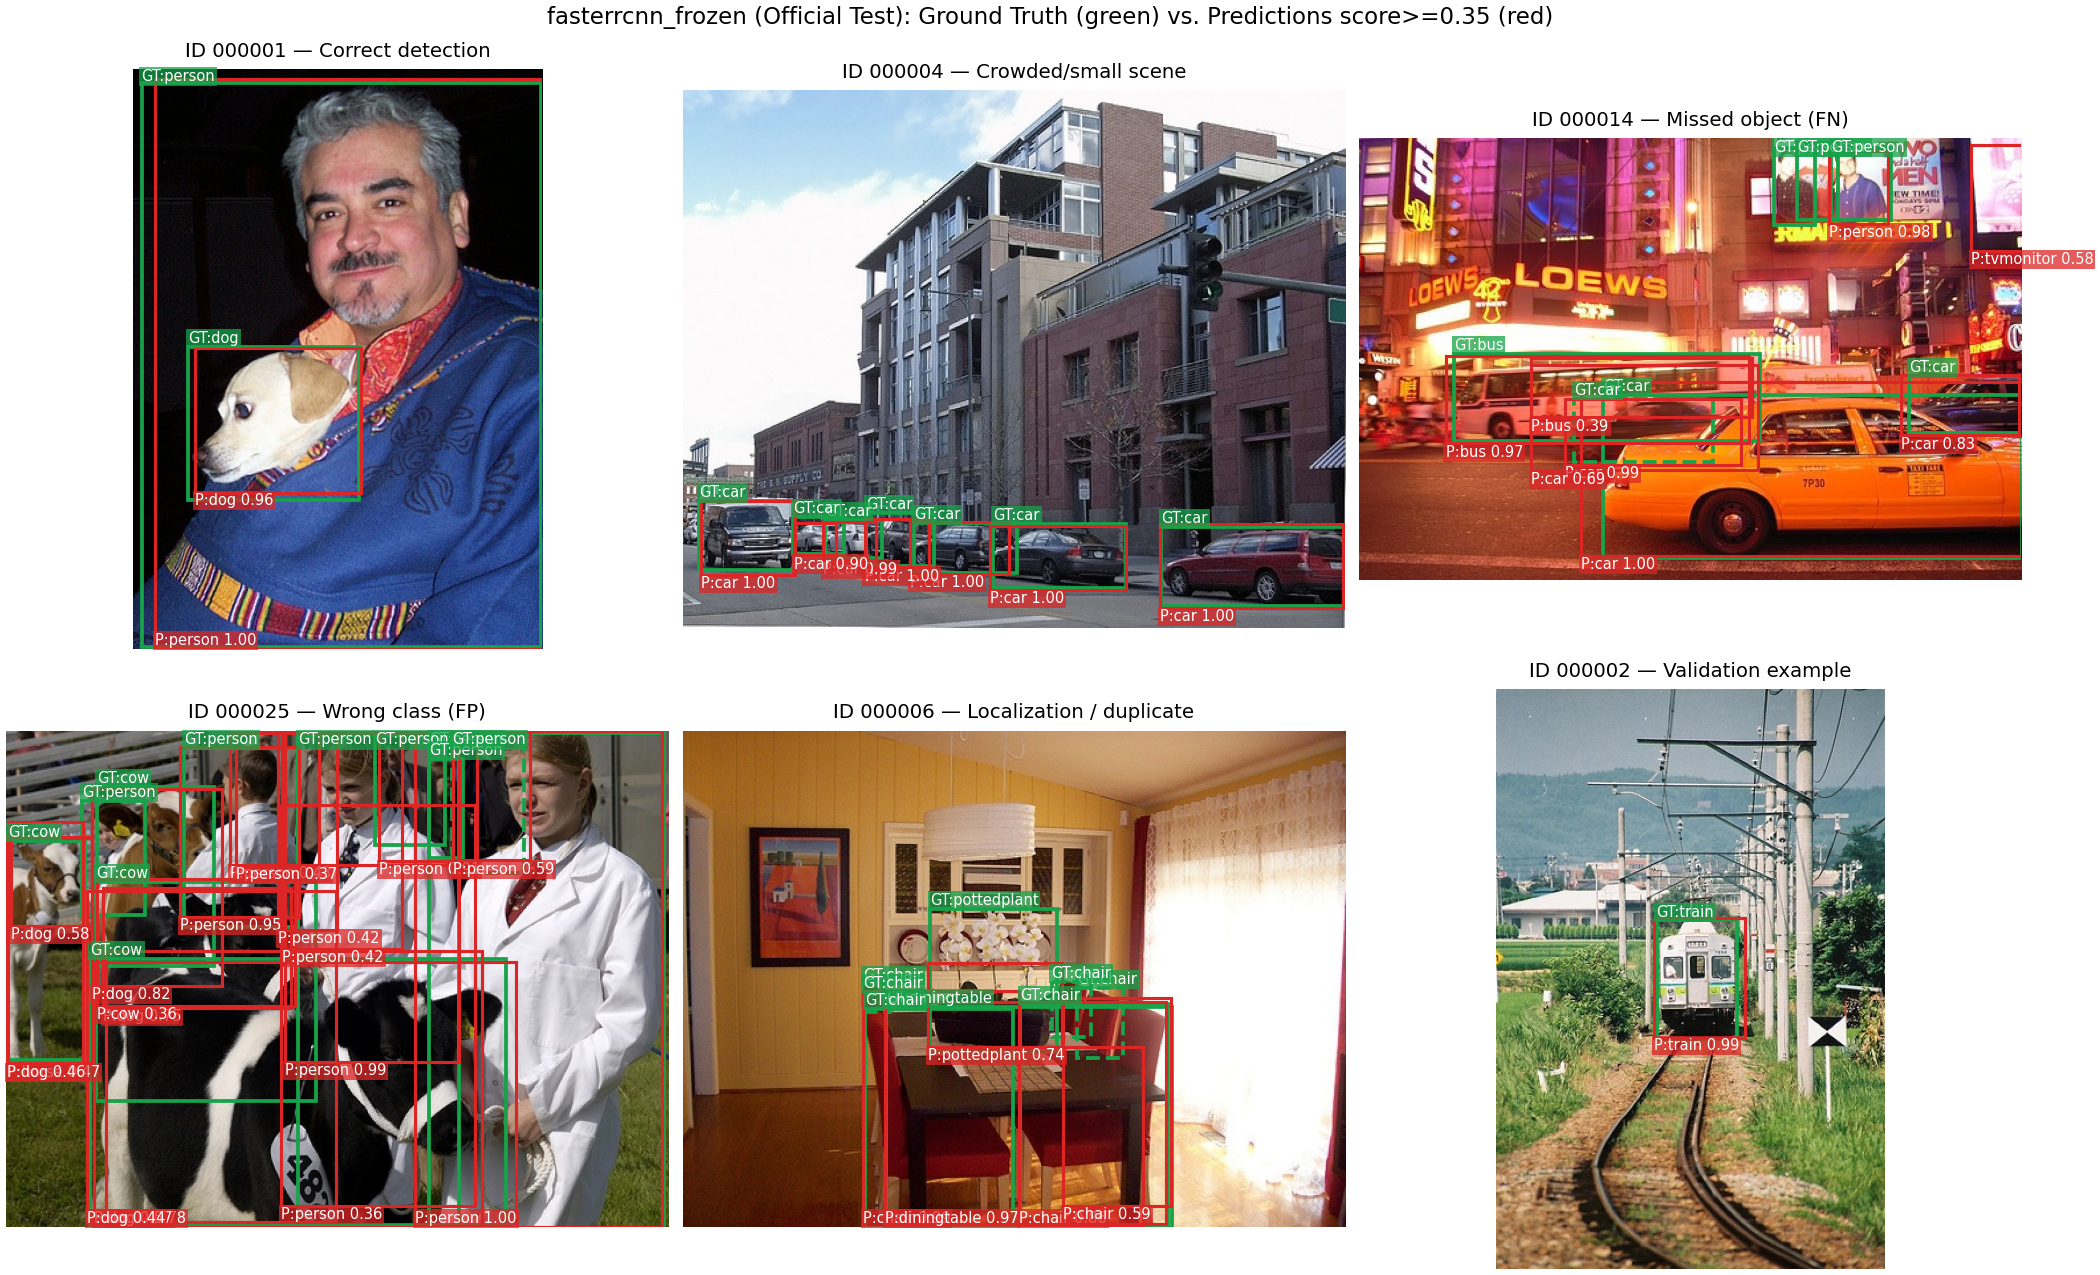
\includegraphics[width=0.90\linewidth]{../../outputs/a2_m3_a100/fasterrcnn_frozen/test_examples.png}
    \caption{\texttt{fasterrcnn\_frozen} qualitative Official Test examples showing strong multi-object recall.}
\end{figure}

\subsection{\textbf{Discussion of Controlled Study and Trade-Offs}}
\begin{enumerate}[itemsep=2pt,topsep=3pt]
    \item \textbf{Why \texttt{fasterrcnn\_frozen} outperforms \texttt{fasterrcnn\_finetune}:} Under a small batch size ($B=2$) and uniform $\text{lr}=0.005$ without warmup, early gradients from the random 21-class \texttt{FastRCNNPredictor} perturb pretrained \texttt{COCO\_V1} ResNet-50 features during epochs 1--8, increasing test wrong-class errors by +32.4\% (1,242 vs. 938) and missing 2.16$\times$ more objects (1,924 vs. 889). Freezing ResNet-50 avoids this drift, cuts peak VRAM by 64.95\% (1,266.2 vs. 3,612.2 MB), and trains 38.2\% faster on L4 (2,425 s vs. 3,926 s).
    \item \textbf{Accuracy--Speed--Memory Trade-Off:} \texttt{ssdlite320} evaluates 4,952 test images in 41.6 s (16.22 ms/img) using 462.8 MB VRAM, but collapses to 0.79\% AP on small test objects (2,151 missed). \texttt{fasterrcnn\_frozen} delivers +30.67 pp higher test mAP at 31.34 ms/img in 1,266.2 MB VRAM.
    \item \textbf{Dominant Semantic Confusions on Test:} Wrong-class errors cluster within indoor furniture (\texttt{sofa $\to$ chair}: 124; \texttt{chair $\to$ sofa}: 45) and animal pairs (\texttt{cat $\to$ dog}: 51; \texttt{dog $\to$ cat}: 40).
\end{enumerate}

\section{Limitations, Conclusion \& AI Usage Disclosure}
\begin{itemize}[itemsep=2pt,topsep=3pt]
    \item \textbf{Limitations:} Single-seed evaluation (\texttt{seed=42}); uniform LR without warmup for full fine-tuning; fixed $320\times320$ resolution bottleneck in \texttt{ssdlite320}.
    \item \textbf{Conclusion:} Combining task-specific EDA, leak-free split grouping (\texttt{000863}/\texttt{008364}), and pretrained FPN features with a frozen ResNet-50 backbone yields \textbf{83.65\% Official Test mAP@0.5} on VOC 2007 while saving nearly two-thirds of training VRAM.
    \item \textbf{AI Usage Disclosure:} AI tools (Google Antigravity, ChatGPT, Claude) assisted with modularizing \texttt{a2/}, implementing the evaluator self-test and overlap audit, and formatting the report. All quantitative results come from executed Colab runs verified by Trần Gia Lâm (2352670) and Nguyễn Hữu Cầu (2352129).
    \item \textbf{Reproducibility \& Artifacts:} Notebook \texttt{notebooks/A2\_M3\_Colab\_Run.ipynb}; Drive checkpoints (\texttt{CO3133\_A2\_M3\_Checkpoints}); video \url{https://youtu.be/OF_lVbQw9zg}.
\end{itemize}

\clearpage
\appendix
\section{Per-Class Official Test AP@0.5 (20 VOC Classes)}
\begin{table}[H]
\centering
\renewcommand{\arraystretch}{0.92}
\resizebox{0.96\linewidth}{!}{%
\begin{tabular}{rlrrrr}
\toprule
\textbf{ID} & \textbf{Category} & \textbf{Test GT} & \textbf{\texttt{ssdlite320}} & \textbf{\texttt{fasterrcnn\_frozen}} & \textbf{\texttt{fasterrcnn\_finetune}} \\
\midrule
1 & aeroplane & 285 & 57.90\% & \textbf{88.68\%} & 85.07\% \\
2 & bicycle & 337 & 63.70\% & \textbf{86.93\%} & 84.20\% \\
3 & bird & 459 & 45.07\% & \textbf{85.71\%} & 73.98\% \\
4 & boat & 263 & 33.16\% & \textbf{72.85\%} & 63.87\% \\
5 & bottle & 469 & 18.31\% & \textbf{81.27\%} & 65.14\% \\
6 & bus & 213 & 64.41\% & \textbf{88.43\%} & 82.01\% \\
7 & car & 1,201 & 63.74\% & \textbf{89.77\%} & 87.58\% \\
8 & cat & 358 & 70.04\% & \textbf{87.19\%} & 82.98\% \\
9 & chair & 756 & 34.04\% & \textbf{73.79\%} & 63.18\% \\
10 & cow & 244 & 44.13\% & \textbf{88.41\%} & 80.34\% \\
11 & diningtable & 206 & 58.46\% & \textbf{78.92\%} & 75.03\% \\
12 & dog & 489 & 65.14\% & \textbf{86.89\%} & 79.75\% \\
13 & horse & 348 & 70.65\% & \textbf{89.85\%} & 85.93\% \\
14 & motorbike & 325 & 62.06\% & \textbf{86.92\%} & 84.23\% \\
15 & person & 4,528 & 60.26\% & \textbf{88.67\%} & 85.88\% \\
16 & pottedplant & 480 & 27.10\% & \textbf{60.25\%} & 51.90\% \\
17 & sheep & 242 & 43.12\% & \textbf{85.27\%} & 73.55\% \\
18 & sofa & 239 & 56.68\% & \textbf{82.05\%} & 77.82\% \\
19 & train & 282 & 70.63\% & \textbf{87.31\%} & 82.14\% \\
20 & tvmonitor & 308 & 50.94\% & \textbf{83.86\%} & 73.53\% \\
\midrule
--- & \textbf{Mean (Official Test mAP@0.5)} & \textbf{12,032} & \textbf{52.98\%} & \textbf{83.65\%} & \textbf{76.90\%} \\
\bottomrule
\end{tabular}%
}
\end{table}

\begin{thebibliography}{9}
\bibitem{everingham2010pascal} M. Everingham, L. Van Gool, C. K. I. Williams, J. Winn, and A. Zisserman, ``The PASCAL Visual Object Classes (VOC) Challenge,'' \textit{IJCV}, vol. 88, no. 2, pp. 303--338, 2010.
\bibitem{ren2015faster} S. Ren, K. He, R. Girshick, and J. Sun, ``Faster R-CNN: Towards Real-Time Object Detection with Region Proposal Networks,'' \textit{NeurIPS}, 2015.
\bibitem{lin2017fpn} T.-Y. Lin, P. Dollár, R. Girshick, K. He, B. Hariharan, and S. Belongie, ``Feature Pyramid Networks for Object Detection,'' \textit{CVPR}, 2017.
\bibitem{howard2019mobilenetv3} A. Howard et al., ``Searching for MobileNetV3,'' \textit{ICCV}, 2019.
\end{thebibliography}

\end{document}
